\documentclass{article}

\usepackage[english]{babel}
\usepackage{amsmath}
\usepackage{amssymb}
\usepackage{amsthm}
\usepackage[font=small]{caption}
\usepackage{cite}
\usepackage{graphicx}

\newtheorem{algorithm}{Algorithm}
\newtheorem{definition}{Definition}
\newtheorem{example}{Example}
\newtheorem{lemma}{Lemma}
\newtheorem{proposition}{Proposition}
\newtheorem{remark}{Remark}

%---------------------------------------------------------------

\title{Analytic combinatorics for bioinformatics: applications to
contig assembly and seeding}
\author{
\textsc{Guillaume Filion} \\ [1ex]
\normalsize CRG, Barcelona
}
\date{\today}

%---------------------------------------------------------------
%---------------------------------------------------------------


\begin{document}

\maketitle

\begin{abstract}
Here is the text of the abstract. I need to type more in order to see if
this goes beyond the two columns of the text.
\end{abstract}


%---------------------------------------------------------------
%---------------------------------------------------------------

\section{Introduction}

How many reads should I sequence? How long should they be? With what
minimum overlap? These questions were first addressed in this context by
Lander and Waterman in a landmark study that defined the ``classic
theory'' of assembly \cite{pmid3294162}, giving estimates of the number of
contigs. At the time, genome assembly was a long term endeavour and it
made sense to gather information about the progress of the project. The
Lander-Waterman estimators are thus accurate for intermediate stages where
the number of contigs is high, but their quality drops when the assembly
nears completion.

Nowadays, genome assembly is several orders of magnitude faster. The
questions remain the same, but in many cases the assembly does not have a
proper intermediate stage because the sequencing capacity of a single run
is potentially sufficient to assemble the target genome. It is thus
desirable to minimize the amount of resources that a necessary for the
task, and estimators that are accurate when assembly is likely to be
possible are generally more useful. Likewise, the parameters of the
algorithm must minimize the risk of misassembly while giving the highest
chance that assembly will be possible. This can be done efficiently only
if the statistical properties of the assembly are also understood when it
is likely to be possible.

These are asymptotic estimates, which means that unlike the classical
estimators, they get more accurate when the number of reads increases. In
practice, they are accurate to within 1\% even for a few hundred reads
taken from a genome of a few hunder nucleotides.

All the results shown here are based on original proofs using analytic
combinatorics \cite{AnalComb2009}. The general strategy of analytic
combinatorics is to (i) describe simple combinatorial objects by a
generating function (ii) use simple mathematical operations to find the
generating function of complex structures based on these objects and (iii)
analyze the singularities of the resulting function to derive asymptotic
estimates. This method is sometimes considered counter-intuitive because
generating functions do not directly appeal to intuition
\cite{AnalComb1996}, but it allows to derive precise estimates with simple
proofs.

Since I expect most readers to not be familiar with analytic
combinatorics, I have tried to introduce the ideas progressively, hoping
that the logic of each step will be apparent. This also means that the
information is somewhat spread throughout the manuscript and does not
clearly separate the biological and the mathematical concepts. I have also
tried to use standard notations from analytic combinatorics for the proofs
of the claims, and standard notations from genomic for the specific
applications, which may be slightly confusing.  The key findings are
applications of recent results of Pemantle and Wilson on multivariate
asymptotics. The reader is referred to the original literature for the
proofs of those theorems \cite{PemWil08,AnalComb2013}.

\textbf{Related work:} Schbath and collaborators \cite{pmid10890387}
studied the effect of varying read length on the distribution of contigs.
Wendl \cite{pmid16901236} developed a theory taking into account ``edge
effects'' appearing when the read length is not negligible compared to the
size of the target genome. Stanhope \cite{pmid20686599} studied the
distribution of the largest contig using models of occupancy.


\section{Results}

\subsection{Analytic combinatorics of the assembly problem}
\label{subsec:config}

\begin{definition}
If $(a_{k,n})_{k \geq 0, n \geq 0}$ is a bivariate array, the generating
function of the array is by definition

\begin{equation*}
A(x,y) = \sum_{k=0}^\infty \sum_{n=0}^\infty a_{k,n}x^ky^n.
\end{equation*}

When $a_{k,n}$ counts the number of objects in a set $\mathcal{A}$, we
will say that $A(x,y)$ is the generating function of those objects, or the
generating function of $\mathcal{A}$. We will refer to $a_{k,n}$ as the
``coefficient of $x^ky^n$ in $A(x,y)$'', and denote it as ``$[x^ky^n]
A(x,y)$'' whenever convenient.

For convenience, we will call the variable associated to $x$ the
\emph{size} and the variable associated to $y$ the \emph{weight}. The
coefficient of $x^ky^n$ in $A(x,y)$ is thus the number of objects in
$\mathcal{A}$ of size $k$ and weight $n$.
\end{definition}

The function $A$ and the bivariate sequence $(a_{k,n})_{k \geq 0, n \geq
0}$ carry the same information, but some combinatorial operations are
easier to perform with $A$, as we will see below.

The first combinatorial object that we will consider is the ``interval'',
defined here as the distance between the left ends of two consecutive
reads. We will call this distance the size of the interval, and we will
impose it to be a strictly positive integer. This means that two reads
cannot map to the same location, but we will later see how to relax this
constraint. We will also give each interval a weight equal to $1$. This
will later allow us to count intervals when we create more complex
objects.

\begin{figure}[h]
\centering
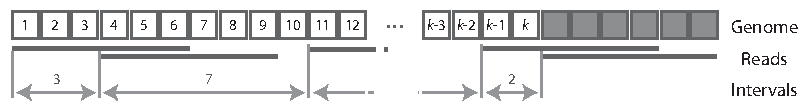
\includegraphics[scale=0.89]{Fig1.pdf}
\caption{\textbf{Representation of the assembly problem}. Here we consider
a single linear chromosome. Reads of identical length are drawn uniformly
without replacement from the chromosome. The distance between the left
ends of consecutive reads forms an interval of requivalent size. We assume
that the leftmost and the rightmost reads always map to the ends of the
chromosome so that intervals always cover exactly $k$ nucleotides.}
\label{fig:sketchass}
\end{figure}

Figure~\ref{fig:sketchass} shows the relationships between reads and
intervals. The ``distance'' between two reads will always be the number of
nucleotides between their left ends, which corresponds to an interval of
the same size. Also note that we assume that the leftmost and the
rightmost nucleotides of the genome are exactly covered by reads. This is
not realistic, but such border effects will have negiligible influence on
the asymptotic estimates.

\begin{remark}
In combinatorics, the coverage of $k$ nucleotides by $n$ intervals
corresponds to a \emph{composition}, \textit{i.e.} the break-down of $k$
as a sum of $n$ positive integers \cite{AnalComb2009}.
\end{remark}

The first question of interest is to know the number of different
configurations for a given value of $k$ and $n$. This problem is simple
enough to showcase the methodology of analytic combinatorics, and the
solution will turn out to be very useful. For now, we observe that we can
``construct'' configurations from intervals.

\begin{definition}
A configuration is a sequence of intervals. The generating function of
configurations is denoted $C(x,y)$.
\end{definition}

The general strategy to count configurations will be to find an expression
for $C(x,y)$, extract its coefficients and find asymptotic estimates for
them. For this, we first need to obtain $I(x,y)$, the generating function
of intervals. For $k > 0$ there is exactly one interval of size $k$ and
weight 1, so the coefficient of $x^ky^n$ equals $1$ if $n = 1$ and $k >
0$, and $0$ otherwise. The generating function of intervals is thus

\begin{equation}
\label{eq:F}
I(x,y) = xy + x^2y + x^3y + \ldots
= xy(1+x+x^2+\ldots) = \frac{xy}{1-x}.
\end{equation}

\begin{remark}
Wherever the equality $1+x+x^2+\ldots = 1/(1-x)$ is used, the condition
$|x| < 1$ is assumed to hold.
\end{remark}

Operations on generating functions allow us to create more complex
combinatorial objects. We have already used additions, which correspond
to disjoint unions. For instance, the generating function above says that
an interval is either an interval of size 1 and weight 1, or an interval
of size 2 and weight 1, or an interval of size 3 and weight 1
\textit{etc}. More generally, if $A(x,y)$ and $B(x,y)$ are the generating
functions of objects in disjoint sets $\mathcal{A}$ and $\mathcal{B}$,
then $A(x,y)+B(x,y)$ is the generating function of objects in $\mathcal{A}
\cup \mathcal{B}$.

Multiplications correspond to Cartesian products. More specifically, if
$A(x,y)$ and $B(x,y)$ are the generating functions of objects in sets
$\mathcal{A}$ and $\mathcal{B}$ (disjoint or not), then $A(x,y)B(x,y)$ is
the generating function of objects in $\mathcal{A} \times \mathcal{B}$.
By doing so, we implicitly assume that the size of $(a,b) \in \mathcal{A}
\times \mathcal{B}$ is the size of $a$ plus the size of $b$, and that the
same goes for the weight.

To prove this identity, observe that the pairs of size $k$ and weight $n$
are made of all pairwise combinations of objects whose sizes sum to $k$
and weights sum to $n$. The number of such pairs is $\sum_{l=0}^k
\sum_{m=0}^n a_{l,m}b_{k-l,n-m}$ so the generating function of pairs is

\begin{equation*}
\begin{split}
\sum_{k=0}^\infty &\sum_{n=0}^\infty \left( \sum_{l=0}^k \sum_{m=0}^n
  a_{l,m}b_{k-l,n-m}\right) x^k y^n \\
&= \sum_{l=0}^\infty \sum_{m=0}^\infty \sum_{k=l}^\infty \sum_{n=m}^\infty
  a_{l,m}b_{k-l,n-m}x^{l + k-l} y^{m + n-m} \\ 
&= \sum_{l=0}^\infty \sum_{m=0}^\infty a_{l,m} x^l y^m
  \sum_{k=l}^\infty \sum_{n=m}^\infty
  b_{k-l,n-m}x^{k-l} y^{n-m} \\
&= B(x,y) \sum_{l=0}^\infty \sum_{m=0}^\infty a_{l,m} x^l y^m
 = A(x,y)B(x,y).
\end{split}
\end{equation*}

% Explain that the size just counts the intervals.
By taking both $\mathcal{A}$ and $\mathcal{B}$ as the set of intervals, we
see that the generating function of pairs of intervals is $I(x,y)^2$.
Applying this formula multiple times, we also see that $I(x,y)^n$ is the
generating function of sequences of $n$ of intervals. Since a sequence of
intervals is either a sequence of $0$ interval, or a sequence of $1$
interval, or a sequence of $2$ intervals \textit{etc}., we can write the
generating function of configurations as

\begin{equation*}
C(x,y) = \sum_{n=0}^\infty \left( \frac{xy}{1-x} \right)^n
= \frac{1}{1 - xy/(1-x)}.
\end{equation*}

\begin{remark}
Note that a sequence of $n$ intervals has weight $n$, so the weight is a
proxy for the number of intervals in the configuration.  We say that $y$
``marks'' the number of intervals.
\end{remark}

We have used $I(x,y)$ to obtain an algebraic expression for $C(x,y)$. The
coefficient of $x^ky^n$ in $C(x,y)$ is the number of configurations where
$n$ intervals cover $k$ nucleotides, but its value does not appear
spontaneously. Fortunately, we can write $C(x,y)$ in such a way that it
will become more obvious. Observe that

\begin{equation}
\label{eq:C}
C(x,y) = \frac{1-x}{1-x(1+y)} =
(1-x) \sum_{k=0}^\infty \left(x(1+y) \right)^k.
\end{equation}


Using Newton's binomial formula, we can expand $(1+y)^k$ so as to extract
the powers of $y$, namely

\begin{equation*}
C(x,y) = (1-x)\sum_{k=0}^\infty x^k\sum_{n=0}^k {k \choose n} y^n
= \sum_{k=0}^\infty\sum_{n=0}^\infty{k \choose n} (x^ky^n - x^{k+1}y^n).
\end{equation*}

It follows that

\begin{equation}
\label{eq:coefC}
[x^ky^n] C(x,y) =
{k \choose n} - {k-1 \choose n} = {k-1 \choose n-1}
\text{, provided $k > 0$, $n > 0$}.
\end{equation}

It can also be seen that the cases $k = 0$ and $n = 0$ give coefficients
equal to $0$, except for $k = n = 0$ where the coefficient is equal to
$1$.

\begin{remark}
The last expression in (\ref{eq:C}) gives an alternative construction for
sequences of intervals. The term $1+y$ is the generating function of bits,
\textit{i.e.} elements of $\{0,1\}$, so $(x(1+y))^k$ is the generating
function of bit strings where $x$ marks the size and $y$ marks the number
of bits set to $1$. To exhibit a bijection we can encode left ends of
intervals with a $1$ and every other position with a $0$. The factor $1-x$
is a correction for the fact that the first bit is always set to $1$ (see
Figure~\ref{fig:sketchass}).
\end{remark}

We now have the \emph{exact} number of configurations for every value of
$k$ and $n$. To obtain asymptotic estimates, we can use Stirling's formula
$n! \sim n^ne^{-n}\sqrt{2\pi n}$. After cancellations we see that the
number of configurations is asymptotically equivalent to

\begin{equation}
\label{eq:assBC}
[x^ky^n]C(x,y) \sim \frac{k^{k-1}}{n^{n-1}(k-n)^{k-n}}
\sqrt{\frac{k}{2\pi n(k-n)}}.
\end{equation}

A more direct approach would have been to observe that a configuration is
a draw of $n-1$ left ends among $k-1$ positions, leading directly to
(\ref{eq:coefC}). The benefit of the analytic combinatorics approach is
that we can now tinker the generating function $C(x,y)$ to obtain results
that do not lend themselves to such direct approaches.




%%%%%%%%%%%%% Average number of contigs %%%%%%%%%%%%%
\subsection{Average number of contigs}
\label{subsec:av}

% ######################################################## %
% Make a note about the fact that they were called islands %
% ######################################################## %

Some configurations are better than others for the purpose of assembling
the genome. In order to investigate the properties of ``good''
configurations, we need to introduce new combinatorial objects.

\begin{definition}
For a given positive integer $d$, an $\alpha$-interval is an interval of
size at most $d$ and an $\omega$-interval is an interval of size greater
than $d$. The generating function of $\alpha$-intervals is denoted
$I_\alpha(x,y)$ and the generating function of $\omega$-intervals is
denoted $I_\omega(x,y)$.
\end{definition}

Intuitively, if two reads are separated by a $\alpha$-interval, it will be
possible to merge them, whereas if they are separated by a
$\omega$-interval this will not be possible. The value of $d$ depends on
the concrete assembly problem at hand and on the read length ($d$ is
higher for longer reads).  This natually lead to the following definition.

\begin{definition}
\label{def:contig}
A contig is a non-empty sequence of $\alpha$-intervals. The generating
function of contigs is denoted $K(x,y)$. A gap is a non-empty sequence of
$\omega$-intervals. The generating function of gaps is denoted $G(x,y)$.
\end{definition}

\begin{figure}[h]
\centering
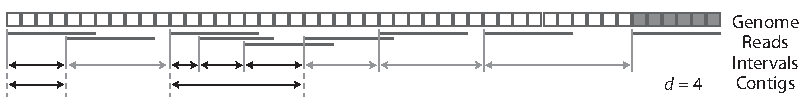
\includegraphics[scale=0.9]{Fig2.pdf}
\caption{\textbf{Contigs and gaps}. In this example $d=4$, so contigs
correspond to sequences of one or more intervals of size at most $4$. The
double arrow is black for $\alpha$-intervals and grey for
$\omega$-intervals. The configuration contains two contigs.}
\label{fig:contigs}
\end{figure}

Note that in real assembly problems, sequencing errors, repeated sequences
and other practical complications may prevent the merging of
$\alpha$-intervals. The properties of the assembly per se depend on the
genome and on the practicalities of the problem at hand.

In order to estimate the expected number of contigs, we start by the
simpler task of estimating the number of $\omega$-intervals. This will
better illustrate the methodolgy, while bringing some useful insight into
the assembly problem.

Following the strategy of analytic combinatorics, we first find the
generating functions of the objects under study. Going back to the
construction of intervals, we can see that the generating functions of
$\alpha$-intervals and $\omega$-intervals are

\begin{equation*}
\begin{split}
I_\alpha(x,y) &= yx + yx^2 + \ldots + yx^d
= yx\frac{1-x^d}{1-x}\text{, and} \\
I_\omega(x,y) &= yx^{d+1} + yx^{d+2} + \ldots = y\frac{x^{d+1}}{1-x}.
\end{split}
\end{equation*}

Observe that $I_\alpha(x,y)+I_\omega(x,y) = I(x,y)$ because an interval is
either an $\alpha$-interval or an $\omega$-interval (and because their
intersection is empty). Using this, we can write the generation of
configurations as

\begin{equation}
\label{eq:C2ndform}
C(x,y) = \sum_{n=0}^\infty I(x,y)^n
= \sum_{n=0}^\infty \left( I_\alpha(x,y) + I_\omega(x,y) \right)^n.
\end{equation}

Since $\omega$-intervals appear explicitly in this expression of $C(x,y)$,
we can use another variable, say $u$, to mark them. For this, we just have
to multiply their generating function by $u$ so that every time an
$\omega$-interval appears in a configuration, the exponent of $u$ is
raised by $1$. The same method was applied earlier to let $y$ mark the
number of intervals. Transforming $C(x,y)$ as described, we obtain

\begin{equation*}
Z(x,y,u) = \sum_{n=0}^\infty \left(xy\frac{1-x^d}{1-x} +
uy\frac{x^{d+1}}{1-x}\right)^n
= \frac{1-x}{1-x-y\left(x(1-x^d) +ux^{d+1}\right)}.
\end{equation*}

$Z(x,y,u)$ is the generating function of a three-dimensional array
$(a_{k,n,m})$, where each term is the number of configurations of total
size $k$, total weight $n$ and with $m$ $\omega$-intervals. Note that both
$\alpha$-intervals and $\omega$-intervals contribute to the weight, so
that it still indicates the number of intervals. For a given value of $k$
and $n$, the cumulative number of $\omega$-intervals is $\sum_{m=0}^\infty
ma_{k,n,m}$. Since for the same values of $k$ and $n$ the total number of
configurations is $\sum_{m=0}^\infty a_{k,n,m}$ the average number of
$\omega$-intervals is

\begin{equation}
\label{eq:average}
\sum_{m=0}^\infty ma_{k,n,m}\Big/\sum_{m=0}^\infty a_{k,n,m}.
\end{equation}

Following the methodology of analytic combinatorics, we will find the
generating functions of the numerator and the denomiator of
(\ref{eq:average}) and extract their respective coefficients. Observe that

\begin{equation*}
\begin{split}
\frac{\partial Z(x,y,u)}{\partial u}\Bigr|_{\substack{\\u=1}} &=
\sum_{k=0}^\infty\sum_{n=0}^\infty
\left(\sum_{m=0}^\infty ma_{k,n,m}\right) x^ky^n \text{, and} \\
Z(x,y,1) &= \sum_{k=0}^\infty\sum_{n=0}^\infty
\left(\sum_{m=0}^\infty a_{k,n,m} \right)x^ky^n.
\end{split}
\end{equation*}

It is easier to start with the generating function of the denominator, as
we already derived the solution. Equation (\ref{eq:C2ndform}) says that
$Z(x,y,1) = C(x,y)$. This is intuitive, because counting
$\omega$-intervals should not change the total number of configurations.
Now turning to the numerator we obtain

\begin{equation*}
\frac{\partial Z(x,y,u)}{\partial u}\Bigr|_{\substack{\\u=1}}
= \frac{yx^{d+1}(1-x)}{\left(1-x(1+y)\right)^2}.
\end{equation*}

There is no obvious way to extract the coefficients of this generating
function. Fortunately, it is close to another generating function for
which we already know the coefficients. Observe that

\begin{equation*}
\frac{\partial C(x,y)}{\partial y} = 
\frac{x(1-x)}{\left(1-x(1+y)\right)^2}.
\end{equation*}

So $\partial Z(x,y,u)/\partial u|_{\substack{\\u=1}} = yx^d\partial
C(x,y)/\partial y$ and the coefficient of $x^ky^n$ in the generating
function of the numrator of (\ref{eq:average}) is $n[x^{k-d}y^n]C(x,y)$.
The average number of $\omega$-intervals is thus

\begin{equation*}
n {k-d-1 \choose n-1} \Big/ {k-1 \choose n-1}.
\end{equation*}

For $k < d$ or $n > k-d$ the average number of $\omega$-intervals is $0$.
We can also use equation (\ref{eq:assBC}) or Sitrling's formula to obtain
a simple asymptotic estimate for the expected number of
$\omega$-intervals, namely

\begin{equation}
\label{eq:avomega}
n\left(1-n/k\right)^d.
\end{equation}

\begin{remark}
Here the benefits of the analytic combinatorics approach become obvious.
It is much more difficult to think of a direct approach leading to this
simple result.
\end{remark}

Recall that this formula assumes that reads cannot map to the same
location. It is possible to filter out identical reads, but it would be
useful to relax this constraint in order to compute estimates before any
data is acquired.

For this, let us assume that we draw $n_*$ reads \emph{with} replacement.
Each nucleotide of the chromosome corresponds to the left end of a read
$n_*/k$ times on average. Because $k$ and $n_*$ are both large, we can
approximate the number of times a nucleotide is drawn by a Poisson
distribution with mean $n_*/k$. The probability that a position is the
left end of a read is approximately $1-e^{-n_*/k}$, so


\begin{equation}
\label{eq:poiss}
n \approx k(1-e^{-n_*/k}).
\end{equation}

\begin{remark}
Allowing intervals and $d$-intervals to have size $0$ is not the proper
way to address this issue because it gives different sampling
probabilities.  For $4$ reads covering $2$ nucleotides the probability
that the first two intervals have size $0$ would be $1/3$, whereas it
should be $2/7$.
\end{remark}

Expression (\ref{eq:avomega}) is useful because at high coverage there
will be approximately one $\omega$-interval between every pair of contigs,
so we can estimate of the average number of contigs as $1 + n(1-n/k)^d$,
using expression (\ref{eq:poiss}) to express $n$ as a function of $n_*$.
However, at low coverage this estimate is inaccurate because there will be
many consecutive $\omega$-intervals not enclosing a contig.

To count the number of contigs more precisely, we can use a slightly more
involved variation of the same strategy. The function $Z(x,y,u)$ above is
a ``counting function'' and $u$ is the ``counting parameter''. We can
count contigs by decorating their generating function with $u$ and again
compute their average number through the ratio

\begin{equation*}
\frac{[x^ky^n] \partial Z(x,y,u)/\partial u|_{\substack{\\u=1}}}
{[x^ky^n]Z(x,y,1)}.
\end{equation*}

All we need to do is find a way to ``construct'' configurations from
contigs and apply the same method as above. It is intuitively clear that
configurations are composed of contigs and gaps, so we need to find the
generating functions of those objects. Contigs are non-empty sequences of
$\alpha$-intervals, so their generating function is

\begin{equation*}
K(x,y) = \sum_{n=1}^\infty \left( I_\alpha(x,y) \right)^n
= \sum_{n=1}^\infty \left(yx\frac{1-x^d}{1-x} \right)^n
= \frac{yx(1-x^d)/(1-x)}{1-yx(1-x^d)/(1-x)}.
\end{equation*}

Similarly, the generating function of gaps is

\begin{equation*}
G(x,y) = \sum_{n=1}^\infty \left(I_\omega(x,y) \right)^n
= \sum_{n=1}^\infty \left(y\frac{x^{d+1}}{1-x} \right)^n
= \frac{yx^{d+1}/(1-x)}{1-yx^{d+1}/(1-x)}.
\end{equation*}

The basic unit of configurations is a contig followed by a gaps. The
generating function of this basic unit is $uK(x,y)G(x,y)$. The presence of
$u$ here indicates that each unit adds 1 to the count of contigs. Finally,
a configuration starts with a potentially empty sequence gap whose
generating function is $1+G(x,y)$, and it ends with a potentially empty
contig, whose generating function is $1+uK(x,y)$. The counting function
thus comes out as

\begin{equation*}
\begin{split}
Z(x,y,u) &= \left( 1+G(x,y) \right)
\left( \sum_{n=0}^\infty (uK(x,y)G(x,y))^n \right)
\left( 1+uK(x,y) \right) \\
& = \frac{(1+G(x,y))(1+uK(x,y))}{1-uK(x,y)G(x,y)}.
\end{split}
\end{equation*}

One can check from the definitions of $K(x,y)$ and $G(x,y)$ that $Z(x,y,1)
= C(x,y)$ as expected. Again, the derivative of $Z(x,y,1)$ is related to
$C(x,y)$, and following the same strategy as before, we obtain

\begin{equation*}
\partial Z(x,y,u)/\partial u|_{\substack{\\u=1}}
= y(1-x^d)\left( 1 - y(x+\ldots+x^d) \right)
\frac{\partial C(x,y)}{\partial y}.
\end{equation*}

The relationship between the coefficients of $\partial Z(x,y,u) /\partial
u|_{\substack{\\u=1}}$ and those of $C(x,y)$ is somewhat cumbersome, but
we still obtain an exact expression for the exepected number of contigs,
namely

\begin{equation*}
\begin{split}
\Bigg[ n{k-1 \choose n-1} - &n{k-d-1 \choose n-1} -
(n-1){k-2 \choose n-2} - \ldots - (n-1) {k-d-1 \choose n-2} +
\\ &(n-1){k-d-2 \choose n-2} +
\ldots + (n-1){k-2d-1 \choose n-2} \Bigg] \Big/ {k-1 \choose n-1}.
\end{split}
\end{equation*}

More interesting is the asymptotic estimate, which comes in a relatively
simple form. The formula above is asymptotically equivalent to

\begin{equation}
\label{eq:avcont}
\left( 1+n(1-n/k)^d \right) \left(1-(1-n/k)^d\right).
\end{equation}

We recognize the previous estimator $1+n(1-n/k)^d$, but here it is
corrected by the factor $1-(1-n/k)^d$, which declines specifically at low
coverage.

Using the Poisson approximation (\ref{eq:poiss}), we can again express the
expected number of contigs as a function of the total number of reads
$n_*$.

Let us now examine a concrete example. In Figure~\ref{fig:avcontig} we
consider a small genome of $k = 25,000$ nucleotides, where $d=24$.
We measure the average number of contigs over
$100,000$ random samples for different number of reads $n_*$ and compare
this value to the Lander-Waterman estimate $n_*e^{-dn_*/k}$
\cite{pmid3294162}, to the Roach estimate $1+(n_*-1)(1-d/k)^{n_*}$
\cite{pmid8808467}, and to the estimate given by formula
(\ref{eq:avcont}).


\begin{figure}[h]
\centering
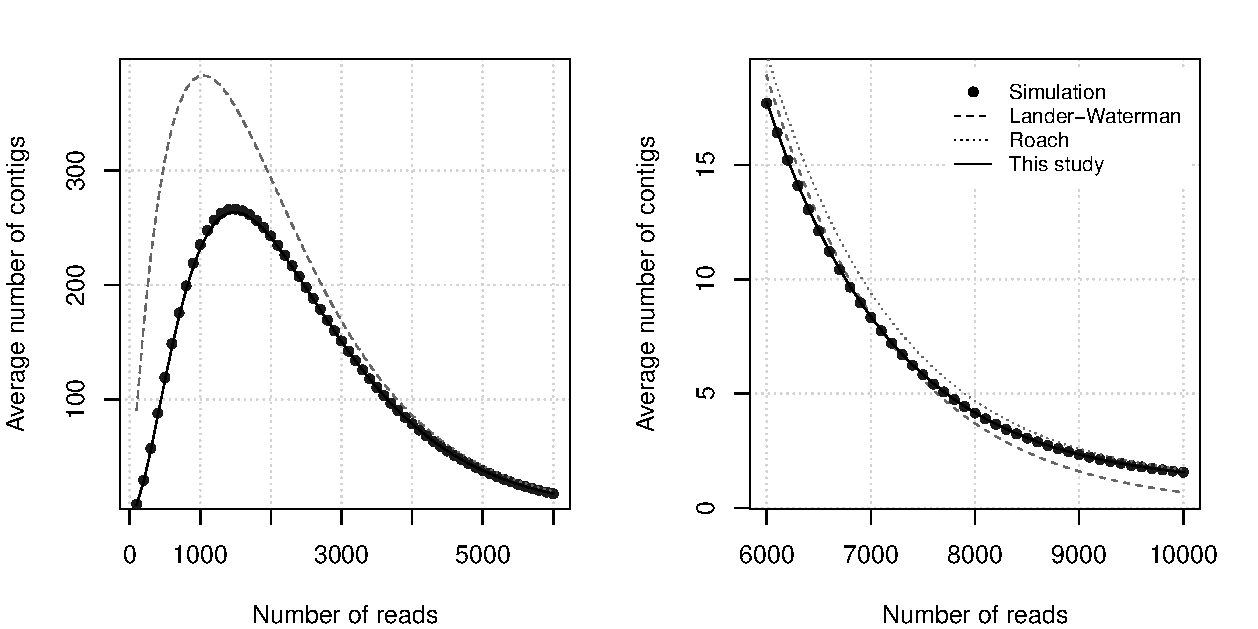
\includegraphics[scale=0.585]{Fig3.pdf}
\caption{\textbf{Average number of contigs}. In this example, $k=25,000$
and $d=24$. Between $100$ and $10,000$ reads were drawn at random with
replacement and the number of contigs was calculated following definition
\ref{def:contig}. Each case was replicated $100,000$ times and the average
was plotted (circles). Dotted lines show the Lander-Waterman and Roach
estimates (the lines are superimposed in the left panel) and the plain
lines show the estimate computed from expression (\ref{eq:avcont}).
The lander-Waterman and Roach estimates are sustantially biased at low
read count (left panel). At high read count (right panel), the Roach
estimate is asymptotically unbiased, but the Lander-Waterman estimate is
not. Here the estimate of this study never deviates by more than 2\%.}
\label{fig:avcontig}
\end{figure}

It is clear that formula (\ref{eq:avcont}) is the most accurate,
especially at low number of reads. The absolute error is largest at the
maximum number of contigs (around $1500$ reads), where the estimate is too
small by approximately $3$ contigs. These small differences do not
disppear for larger values of $k$, they are due to the Poisson
approximation (\ref{eq:poiss}), which brings small but systematic biases.

In conclusion, we have obtained an estimator that is accurate at all
values of the coverage. It was derived using the standard analytic
combinatorics approach and that it involves only basic mathematical
manipulations.





%%%%%%%%%%%%% Probability of closure %%%%%%%%%%%%%
\subsection{Probability of closure}
\label{subsec:closure}

An important factor in the assembly problem is whether the read coverage
will be tight enough to reconstruct whole chromosomes, \textit{i.e.}
whether the configuration consists of a single contig without gap. To
answer this question, we introduce the concept of ``closure''.

\begin{definition}
\label{def:closure}
A closed configuration is such that all intervals are $\alpha$-intervals.
\end{definition}

The probability of closure is the number of closed configurations divided
by the total number of configurations. As before, we will use generating
functions to count both types of configurations, and use asymptotic
estimates of their coefficients to compute the probability.

The generating function of configurations is $C(x,y)$, as we have seen
multiple times. Closed configurations are simple contigs, so their
generating function is $K(x,y)$, defined in section (\ref{subsec:avctsz}).
The the probability we are looking for is thus

\begin{equation*}
\frac{[x^ky^n]K(x,y)}{[x^ky^n]C(x,y)}.
\end{equation*}

Unfortunately, we cannot extract the coefficients of $K(x,y)$. These
numbers are known as the ``polynomial coefficients'', but they cannot be
expresssed in a simple form. However, it is usually impossible to obtain
an extact expression for the coefficients of a generating function. We
were ``lucky'' in the previous examples, but luck is not necessary.  The
asymptotic behavior of the coefficients is entirely captured by the
generating function and it can be extracted in a nearly automatic way. We
will now see how to do this with more advanced analytic combinatorics
tools.

\begin{definition}
Riordan arrays are bivariate arrays $(a_{k,n})$ whose generating
function can be written as

\begin{equation}
\label{eq:RAGF}
\sum_{k=0}^\infty \sum_{n=0}^\infty a_{k,n} x^k y^n =
\frac{\phi(x)}{1-y \nu(x)}.
\end{equation}

For simplicity, we will refer to generating functions of Riordan arrays
as ``Riordan generating functions''.
\end{definition}

Configurations form a Riordan array because $C(x,y)$ can be written as
(\ref{eq:RAGF}) by setting $\phi(x) = 1$ and $\nu(x) = x/(1-x)$.
Potentially empty contigs also form a Riordan array because the generating
function $1+A(x,y)$ can be written as (\ref{eq:RAGF}) by setting $\phi(x)
= 1$ and $\nu(x) = x+x^2+\ldots+x^d = x(1-x^d)/(1-x)$.

The aymptotic behavior of Riordan arrays can be extracted from their
generating function by the following theorem of Pemantle and Wilson.

\begin{proposition}
\label{th:PW}
Assume that $F(x,y)$ is the generating function of a Riordan array, and
that $k$ and $n$ tend to infinity with $\lim k/n = \lambda$, then

\begin{equation}
\label{eq:assRA}
[x^ky^n]F(x,y) \sim \frac{\nu(x_*)^n\phi(x_*)}
  {x_*^k\sqrt{2\pi n \sigma(x_*)^2}},
\end{equation}

\noindent
where $x_*$ is the solution of the equation $\mu(x) =
x\nu'(x)/\nu(x) = \lambda$ and where $\sigma(x)^2$ is the function $x
\mu'(x)$. We will call $x_*$ the critical value associated with $k$ and
$n$.
\end{proposition}

The proof of this theorem is outside the scope of this manuscript;
interested readers are referred to the original results of Pemantle and
Wilson \cite{PemWil02,AnalComb2013}.

In essence, proposition \ref{th:PW} says that if we can find the critical
values of the generating function, then we get the asymptotic growth of
the Riordan array. The following lemma shows that this is realitvely easy
in the case of
$A(x,y)$.

\begin{lemma}
\label{th:mu}
Riordan generating functions where $\nu(x) = a(x) = x+x^2+\ldots+x^d$
have only one critical value $x_a$ for $1 \leq \lambda \leq d$.
\end{lemma}

\begin{proof}
We first demonstrate that for $x \geq 0$, the function $\mu$ is
strictly increasing. This will ensure that if the solution is unique if
it exists.

\begin{equation}
\label{eq:mu}
\mu_a(x) = x\frac{a'(x)}{a(x)} =
\frac{x+2x^2+3x^3+\ldots+dx^d}{x+x^2+\ldots+x^d} =
d+\frac{1}{1-x} - \frac{d}{1-x^d}.
\end{equation} 

Differentiating the last expression we obtain

\begin{equation}
\label{eq:muprime}
\mu_a'(x) = \frac{1}{(1-x)^2} -\frac{d^2x^{d-1}}{(1-x^d)^2}.
\end{equation}

The function $f(\alpha) = x^{\alpha} = e^{\alpha \log(x)}$ is strictly
convex for every $x > 0$ and $x \neq 1$. Applying the definition of
convexity, we obtain the inequality

\begin{eqnarray*}
\frac{f(0)+\ldots+f(d-1)}{d} &>&
f\left(\frac{0+1+2+\ldots+d-1}{d}\right) \text{, and then} \\
\frac{1+x+\ldots+x^{d-1}}{d} &>& f\left(\frac{d-1}{2}\right)
= x^{(d-1)/2} \\
\frac{1-x^d}{1-x} &>& dx^{(d-1)/2} \\
\frac{1}{(1-x)^2} &>& \frac{d^2x^{d-1}}{(1-x^d)^2}.
\end{eqnarray*}

Combined with equation (\ref{eq:muprime}), the last inequality shows that
$\mu_a'(x) > 0$ for $x > 0$ and $x \neq 1$. Since $\mu_a'(0) = 1$ and
$\mu_a'(1) = (d+1)(d-1)/12$, $\mu_a$ is strictly increasing (note that
$\mu_a'(1)$ is properly defined but that $\mu_a'(0)$ must be defined by
continuity).  Observing that $\mu_a(0) = 1$ and
$\lim_{x\rightarrow\infty} \mu_a(x) = d$, the equation
$\mu_a(x) = \lambda$ has a unique solution
provided $1 \leq \lambda \leq d$.
\end{proof}

\begin{remark}
The cases $\lambda < 1$ and $\lambda > d$ correspond to limits where $nd <
k$ and $n > k$, respectively. Since the size of a collection of $n$
$d$-intervals is between $n$ and $nd$, we have the trivial asymptotic
behavior $[x^ky^n]A(x,y) = 0$ in both cases.
\end{remark}


The value of $x_a$ can be found numerically from expression
(\ref{eq:mu}).  Once it is available, we can compute $\nu(x_a)$ and
$\sigma_a(x_a)^2$ from their definitions, but numeric precision can
become an issue if $n$ or $d$ is very large. To avoid this, we can use the
equivalent expressions


\begin{gather}
\label{eq:nu} %% Equation for nu.
a(x_a) = \frac{dx_a}{1+(d-\lambda)(1-x_a)}, \\
\label{eq:sigma} %% Equation for sigma2.
\sigma_a(x_a)^2 = \lambda(d-\lambda) -
  \frac{d-2\lambda+1}{1-x_a}.
\end{gather}

As above, we need to replace $n$ by its estimate from the Poisson
approximation (\ref{eq:poiss}) because the weight $n$ is determined by the
number of distinct reads.


\begin{algorithm}
\label{alg:closure}

Here are the steps required to compute the probability of obtaining a
closed configuration for a genome of size $k$, with required overlap $d$
and with $n_*$ reads.

\begin{enumerate}
\item Compute $n = k(1-e^{-n_*/k})$
\item Compute $\lambda = k/n$
\item Solve $\mu_a(x_a) = \lambda$ by the Newton-Raphson method using
(\ref{eq:mu}) and (\ref{eq:muprime})
\item Compute $a(x_a)$ and $\sigma_a^2(x_a)$ using
(\ref{eq:nu}) and (\ref{eq:sigma})
\item Compute (\ref{eq:assRA}) in logarithmic space
\item Compute (\ref{eq:coefC}) in logarithmic space
\item Take the difference of the last two terms and exponentiate.
\end{enumerate}

Few Newton-Raphson iterations are required for convergence (less than ten)
and the whole process completes in tens of microseconds or less on most
computers.

We illustrate this method on a genome with $k = 25000$, and assembly
conditions where $n_* = 10000$ and $d=24$. Using the Poisson
approximation, we obtain $n \approx 25000 \cdot (1-e^{-10000/25000})
\approx 8241.9988$.

From this, we obtain $\lambda = k/n \approx 3.033$. Using the
Newton-Raphson method with expressions (\ref{eq:mu}) and
(\ref{eq:muprime}), we solve the equation $\mu(x_a) = \lambda$ and obtain
$x_a \approx 0.67049776$. Using equations (\ref{eq:nu}) and
(\ref{eq:sigma}), we obtain $a(x_a) \approx 2.03474206$ and
$\sigma_a(x_a)^2 \approx 6.136354$. Computing (\ref{eq:assRA}) in
logarithmic space with the new values yields

\begin{equation*}
\begin{split}
8241.9988\log(2.03474206) - &25000\log(0.67049776) \\
- \log(8241.9988)/2 - &\log(6.136354)/2 - \log(2\pi)/2
\approx 15841.899.
\end{split}
\end{equation*}

We compute the number of configurations in logarithmic space from equation
(\ref{eq:coefC}) and obtain

\begin{equation*}
\log { 24999 \choose 8240.9988 } \approx 15842.457.
\end{equation*}

Finally, the estimated probability that a configuration is closed for a
genome of size $k=25000$, with coverage $n_* = 10000$ reads and
$24$-intervals is

\begin{equation*}
\exp(15842.084-15842.457) \approx 0.573.
\end{equation*}


\end{algorithm}


Figure~\ref{fig:closureprob} expands the example given at the end of
section \ref{subsec:av}, where $k = 25,000$ nucleotides and where $d=24$.
The Roach estimate is $(1-(1-d/k)^n)^{n-1}$ \cite{pmid8808467}.

\begin{figure}[h]
\centering
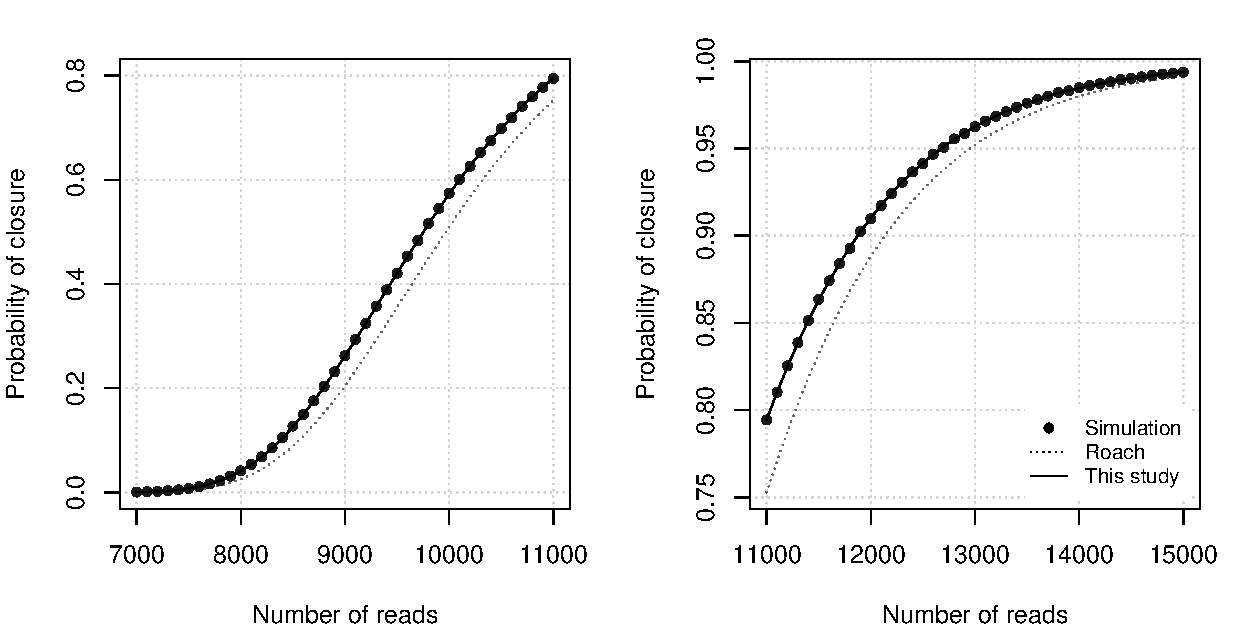
\includegraphics[scale=0.585]{Fig4.pdf}
\caption{\textbf{Probability of closure}. In this example, $k=25,000$ and
$d=24$. Between $7,000$ and $15,000$ reads were drawn at random with
replacement and closure was determined following definition
\ref{def:closure}. Each case was replicated $500,000$ times and the
average frequency of closure was plotted (circles). Dotted lines show the
Roach estimate and the plain lines show the estimate computed with
algorithm \ref{alg:closure}. At its worst, the Roach estimate is off the
target value by approximately 0.07, whereas the analytic combinatorics
estimate never deviates by more than 0.002.}
\label{fig:closureprob}
\end{figure}




%%%%%%%%%%%%% Probability of m contigs %%%%%%%%%%%%%
\subsection{Probability of $m$ contigs}
\label{subsec:probmcontigs}

We now turn our attention to a problem that will illustrate how we can
combine generating functions of Riordan arrays to describe more complex
combinatorial objects. The aim is to compute the probability that the
configuration consists of a given number of contigs $m$.

We start with the special case $m = 0$, which is handled differently from
the others. A configuration contains $0$ contig if all the intervals are
$\omega$-intervals, or in other words, if the configuration is a breach.
Recall from section \ref{subsec:av} that the generating function of
breaches is

\begin{equation*}
B(x,y) = \sum_{n=1}^\infty \left( \frac{yx^{d+1}}{1-x} \right )^n.
\end{equation*}

The coefficient of $x^ky^n$ in $B(x,y)$ is thus equal to the coefficient
of $x^k$ in $\left(x^{d+1}/(1-x)\right)^n$, or alternatively, the
coefficient of $x^{k-dn-n}$ in $1/(1-x)^n$. From the Taylor expansion of
$1/(1-x)^n$, this coefficient is seen to be equal to ${k-dn-1 \choose
n-1}$. The probability that the configuration contains eactly $0$ contig
is thus

\begin{equation}
\label{eq:m=0}
{k-dn-1 \choose n-1} \Big/ {k-1 \choose n-1} \sim 
\frac{(k/n)^{k-1/2}(k/n-d)^{k-dn-1/2}}
 {(k/n-1)^{k-n+1/2}(k/n-d-1)^{k-(d+1)n-1/2}}.
\end{equation}

Proposition \ref{th:PW} gives the asymptotic growth directly, but the
approach above exhibits the exact solution. For $m > 0$, the exact
solution will be not available because the generating functions are
more complex.

A configuration with $m$ contigs must also contain at least $m-1$
breahes, plus up to two additional breaches at the ends. The generating
functions of breaches, potentially empty breaches and contigs are
$B(x,y)$, $1+B(x,y)$ and $A(x,y)$, respectively. Since a configuration
with $m$ contigs is an alternating sequence of those objects, the
generating function appears as

\begin{equation*}
\begin{split}
K(x,y) &= (1+B(x,y)) A(x,y) B(x,y) A(x,y) \ldots A(x,y) (1+B(x,y)) \\
&= \frac{y^ma(x)^m}{(1-ya(x))^m}
\frac{y^{m-1}b(x)^{m-1}}{(1-yb(x))^{m+1}}.
\end{split}
\end{equation*}

$K(x,y)$ is not a Riordan generating function, but it can be transformed
so as to allow us to use proposition \ref{th:PW}. More specifically,
$K(x,y)$ can be written as the double sum

\begin{equation}
\label{eq:mcontigs}
K(x,y) = A_*(x,y) + B_*(x,y) =
\sum_{j=0}^m\frac{\alpha_j(x)}{\left(1-ya(x)\right)^j}
+ \sum_{j=0}^{m+1}\frac{\beta_j(x)}{\left(1-yb(x)\right)^j}.
\end{equation}

If we fix $x$, $F(x,y)$ appears as a rational function of $y$, so using
standard methods, we can see that $\alpha_m(x) = (b(x)/a(x))^{m-1} /
(1-b(x)/a(x))^{m+1}$, and that $\beta_{m+1}(x) = (a(x)/b(x))^m /
(1-a(x)/b(x))^m$. With these explicit formulas, we can write $F(x,y)$ as

\begin{equation}
\label{eq:mcontigs_epsilon}
\frac{x^{d(m-1)}(1-x^d)^2}{(1-2x^d)^{m+1}}
  \frac{1}{\left(1-ya(x)\right)^m} + 
\frac{(1-2x^d)^m}{x^{dm}}
  \frac{1}{\left(1-yb(x)\right)^{m+1}} + \varepsilon(x,y),
\end{equation}

\noindent
where $\varepsilon(x,y)$ involves lower powers of $1 / (1-ya(x))$ and
$1 / (1-yb(x))$. The lemma below shows that we can extract the coefficient
asymptotics from this expression and that $\varepsilon(x,y)$ does not
contribute to the leading term.

\begin{lemma}
\label{lem:RAasspow}
Assume that the generating function $F_j(x,y)$ can be written as

\begin{equation*}
F_j(x,y) =
\frac{\phi(x)}{(1-y\nu(x))^j}.
\end{equation*}

If $k$ and $n$ tend to infinity with $\lim k/n = \lambda$, then

\begin{equation}
\label{eq:RAasspow}
[x^ky^n]F_j(x,y) \sim {n-j+1 \choose j-1}
\frac{\nu(x_*)^n \phi(x_*)}
{x_*^k\sqrt{2\pi n \sigma(x_*)^2}},
\end{equation}

\noindent
where $x_*$ is the critical value, \textit{i.e.} the solution of
$\mu(x) = x\nu'(x)/\nu(x) = \lambda$ and $\sigma(x)^2 = x \mu'(x)$,
as in proposition \ref{th:PW}.
\end{lemma}

\begin{proof}
Define the Riordan generating function $G(x,y)$ as

\begin{equation*}
G(x,y) = \frac{\phi(x)}{1-y\nu(x)} =
\sum_{k=0}^\infty\sum_{n=0}^\infty a_{k,n} x^ky^n.
\end{equation*}

Differentiate the equality above $j-1$ times with respect to $y$ to
obtain

\begin{equation*}
\begin{split}
\frac{\partial^{m-1} G(x,y)}{\partial y^{m-1}} &=
\sum_{k=0}^\infty\sum_{n=0}^\infty n(n-1)\ldots(n-j+2)
a_{k,n} x^ky^{n-m+1} \\
&= (j-1)!\frac{\phi(x)\nu(x)^{n-1}}{(1-y\nu(x))^m}
= (j-1)!\nu(x)^{m-1}F_j(x,y).
\end{split}
\end{equation*}

This shows that the coefficients of $F_j(x,y)$ are related to the
coefficients of $G(x,y)$ by the equality

\begin{equation*}
[x^ky^n]F_j(x,y) = \frac{1}{\nu(x)^{m-1}} {n+j-1 \choose j-1}
  [x^ky^{n+m-1}]G(x,y).
\end{equation*}

Since $G(x,y)$ is a Riordan generating function, apply proposition
\ref{th:PW} and simplify to obtain (\ref{eq:RAasspow}).
\end{proof}

Lemma \ref{lem:RAasspow} shows that we can obtain the asymptotic behavior
of the coefficients of (\ref{eq:mcontigs}) as a sum of $2m-1$ terms, but
it also shows that the coefficients of $\varepsilon(x,y)$ are
asymptotically negligible. Indeed, the critical value of $F_j(x,y)$
is the same for every value of $j$, so according to equation
(\ref{eq:RAasspow}), the coefficients of $F_j(x,y)$ are
$O(1/n)$ compared to the coefficients of $F_{j+1}(x,y)$.

Recall that $x_a$ denotes the critical value of $A(x,y)$. Similarly, we
denote $x_b$ the critical value of $B(x,y)$. With these notations, the
asymptotic behavior of the coefficients of $K(x,y)$ appears as

\begin{equation}
\label{eq:nasty}
\begin{split}
[x^ky^n]K(x,y) \sim {n-m+1 \choose m-1 }
    &\frac{(1-x_a^d)^2}{(1-2x_a^d)^{m+1}}
    \frac{a(x_a)^n} {x_a^{k-d(m-1)}\sqrt{2\pi n \sigma_a(x_a)^2}} \\
 + {n-m \choose m} &(1-2x^d)^m
    \frac{b(x_b)^n} {x_b^{k+dm}\sqrt{2\pi n \sigma_b(x_b)^2}}.
\end{split}
\end{equation}

We can expect that equation (\ref{eq:mcontigs_epsilon}) will have three
asymptotic regimes. In the case that $x_a > x_b$ and $a(x_a) > b(x_b)$,
the coefficients of $B_*$ are exponentially small compared to the those of
$A_*$, so they can be neglected. The converse is also true. But if $x_a >
x_b$ and $a(x_a) < b(x_b)$, or if $x_a < x_b$ and $a(x_a) > b(x_b)$, then
none of the functions can be neglected, and the coefficients have ``mixed
asymptotics''. Pemantle and Wilson \cite{AnalComb2013} formalize this
concept and explain how to distinguish these cases, but here we will
simply use formula (\ref{eq:nasty}) without discrimination.


\begin{algorithm}
\label{alg:nasty}

Here are the steps required to compute the probability of obtaining a
configuration with $m$ contigs for a genome of size $k$, with required
overlap $d$ and with $n_*$ reads.

\begin{enumerate}
\item Compute $n = k(1-e^{-n_*/k})$
\item Compute $\lambda_1 = (k-d(m-1))/n$
\item Solve $\mu_a(x_a) = \lambda_1$ by the Newton-Raphson method using
(\ref{eq:mu}) and (\ref{eq:muprime})
\item Compute $a(x_a)$ and $\sigma^2(x_a)$ using
(\ref{eq:nu}) and (\ref{eq:sigma})
\item Compute $\lambda_2 = (k+dm)/n$
\item Compute $x_b = (\lambda_2-2)/(\lambda_2-1)$
\item Compute $b(x_b) = (\lambda_2-2)^{d+1} / (\lambda_2-1)^d$
and $\sigma_b(x_b)^2 = (\lambda_2-2)(\lambda_2-1)$
\item Compute the two terms of (\ref{eq:nasty}) in logarithmic space
\item Compute (\ref{eq:coefC}) in logarithmic space
\item Take the differences, exponentiate and sum.
\end{enumerate}

We illustrate this method to compute the probability that the
configuration has $m=10$ contigs on a genome with $k = 25000$, and
assembly conditions where $n_* = 7000$ and $d=24$. Using the Poisson
approximation, we obtain $n \approx 25000 \cdot (1-e^{-7500/25000})
\approx 6105.4065$.

From this, we obtain $\lambda_1 = (k-d(m-1))/n \approx 4.0593$. Using the
Newton-Raphson method with expressions (\ref{eq:mu}) and
(\ref{eq:muprime}), we solve the equation $\mu(x_a) = \lambda_1$ and
obtain $x_a \approx 0.75538011$. Using equations (\ref{eq:nu}) and
(\ref{eq:sigma}), we obtain $a(x_a) \approx 3.08429680$ and
$\sigma_a(x_a)^2 \approx 11.93581488$. The first term of
(\ref{eq:nasty}) in logarithmic space is thus approximately equal to

\begin{equation*}
\begin{split}
\log { 6096 \choose 9 } &+ 2\log(1-0.75538011^d)
-11\log(1-2\cdot0.75538011^d) \\
&+ 6105.4065\log(3.08429680) - 24784\log(0.75538011) \\
&- \log(6105.4065)/2 - \log(11.93581488)/2 - \log(2\pi)/2
\approx 13888.583.
\end{split}
\end{equation*}

We also obtain $\lambda_2 = (k+dm)/n \approx 4.1340$. This directly yields
$x_b \approx 0.68092311$, $b(x_b) \approx 0.00021065$, and
$\sigma_b(x_b)^2 \approx 6.68817131$. The second term of (\ref{eq:nasty})
in logarithmic space is thus approximately equal to

\begin{equation*}
\begin{split}
\log { 6097 \choose 10 } &+ 10\log(1-2\cdot0.68092311^d) \\
&+ 6105.4065\log(0.00021065) - 25240\log(0.68092311) \\
&- \log(6105.4065)/2 - \log(6.68817131)/2 - \log(2\pi)/2
\approx 9757.229.
\end{split}
\end{equation*}

The second term is much smaller than the first so it can be neglected.
We compute the number of configurations in logarithmic space from equation
(\ref{eq:coefC}) and obtain

\begin{equation*}
\log { 24999 \choose 6104.4065} \approx 13890.737.
\end{equation*}

Finally, the estimated probability that a configuration is closed for a
genome of size $k=25000$, with coverage $n_* = 10000$ reads and
$24$-intervals is

\begin{equation*}
\exp(13888.583-13890.737) \approx 0.116
\end{equation*}


\end{algorithm}


%%%%%%%%%%%%% Average contig size %%%%%%%%%%%%%
\subsection{Average contig size}
\label{subsec:avctsz}

Another feature of interest is the average size of the contigs. However
tempting to estimate it as the ratio of the expected cumulative contig
size and the expected number of contigs, this method is inaccurate. The
number of contigs and their cumulative size are not statistically
independent, so the expected value of their ratio is not equal to the
ratio of their expected values. We need a more sophisticated estimator.

For this, we will use the counting function of contigs, to which we are
will add a counter for the size of contigs. Following the method used to
count contigs in subsection \ref{subsec:av}, the function that counts
both contigs and their cumulative size is

\begin{equation*}
\begin{split}
Z(x,y,u,z) = \frac{(1+G(x,y))(1+uK(zx,y))}{1-uK(zx,y)G(x,y)}.
\end{split}
\end{equation*}

The variable $z$ counts the cumulative size of contigs (and as before, the
variable $u$ counts their number). The exponent of $x$ marks the total
size of a configuration, and it is obvious that the exponent of $z$ in
this function marks the ``amount of size'' allocated to contigs.
$Z(x,y,u,z)$ is the generating function of a four-dimensional array
$(a_{k,n,m,p})$, where each term is the number of configurations of size
$k$ and weight $n$, and with $m$ contigs of cumulative size $p$.

As in subsection \ref{subsec:av}, averaging will reduce the number of
variables to two, and we will need to extract the coefficients of a
bivariate generating function. The average contig size of configurations
of size $k$ and weight $m$ is

\begin{equation*}
\sum_{m=1}^\infty\frac{1}{m}\sum_{p=0}^\infty pa_{k,n,m,p}.
\end{equation*}

So the counting function of the average contig size is found by first
differentiating $Z(x,y,u,z)$ with respecto to $z$ and then integrating
with respect to $u$. More specifically, the function we are looking for is

\begin{equation*}
H^*(x,y) = \int \frac{1}{u}
\frac{\partial Z(x,y,u,z)}{\partial z}\Bigr|_{\substack{\\z=1}} du
\biggr|_{\substack{\\u=1}}.
\end{equation*}

We now proceed as obvious.

\begin{equation*}
\begin{split}
\frac{\partial Z(x,y,u,z)}{\partial z} &=
\frac{xu\left(1+G(x,y)\right)^2 \partial K(zx,y)/ \partial x}
{\left(1-uK(zx,y)G(x,y)\right)^2} \text{, and} \\
H^*(x,y) &=  x \frac{\partial K(x,y)}{\partial x}
\frac{\left(1+G(x,y)\right)^2}{1-K(x,y)G(x,y)}.
\end{split}
\end{equation*}

In the derivation above, it is important to choose the integration
constant such that the coefficient of $u^0$ is $0$ so that the average
contig size of a configuration without contig is $0$. Rearranging the
terms, we obtain

\begin{equation*}
\begin{split}
H^*(x,y) &= x \frac{\partial K(x,y)}{\partial x}
\frac{1+G(x,y)}{1+K(x,y)}C(x,y) \\
&= \frac{yx(1-(d+1)x^d+dx^{d+1})(1-x)^3}
{\big(1-x-yx(1-x^d)\big)\big(1-x-yx^{d+1}\big)\big(1-x-yx\big)}.
\end{split}
\end{equation*}




\section{Seeding}

Computing the best alignment between two sequences is carried out by
dynamic programming. However, the running time of these algorithms scale
$O(mn)$, where $m$ and $n$ are the sequence lengths, so it is only
feasible for short sequences. For long sequences, heuristics are used for
speed up, and the most popular by far belong to ``seeding'' methods.



\section{Discussion}

Strictly speaking, we do not need the theorems by Pemantle and Wilson.
Here we care only about approximations rather than asymptotics. We could
have used earlier results by Drmota \cite{Drmota1994} or Gardy
\cite{Gardy1995}, or we could have used the saddle point asymptotics
method on $(x(1-x^d)/(1-x))^n$ we would obtain expression (\ref{eq:assRA})
for fixed $n$ and $k$, which is sufficient for our purpose. However, this
would have required to check that the function satisfies some conditions
that are fairly technical. Proposition \ref{th:PW} is very general and it
makes this step unnecessary.

\section{Appendix}

Occasionally, we need the second order term of the asymptotics. In the
case of Riordan arrays, it is not so difficult to find it.

\begin{proposition}
With the same assumptions and notations as proposition \ref{th:PW}

\begin{equation}
[x^ky^n]F(x,y) \sim \frac{\nu(x_\lambda)^n\phi(x_\lambda)}
  {x_\lambda^k\sqrt{2\pi n \sigma(x_\lambda)^2}}
\left(1-\left(\frac{15}{8}c_3^2+\frac{3}{2}c_4\right)
\frac{1}{n\sigma(x_\lambda)^2} \right),
\end{equation}

\noindent
where $\varphi(\theta) = -\log \nu(x_\lambda e^{i\theta}) - c_0
-c_1\theta = c_2\theta^2 + c_3\theta^3 + c_4\theta^4 + O(\theta^5)$.
\end{proposition}

This result is implicitly proved in \cite{AnalComb2013}.
For Riordan arrays, the function $A(\theta)$ of formula (9.2.9) in
is equal to $-1$. The integral of proposition 9.2.5
thus reduces to $\int_{N'}e^{-n\varphi(\theta)}d\theta$ and the
coefficients can be computed from the proof of theorem 4.1.1. Note that 
$c_2 = \sigma(x_\lambda)^2/2$.

%---------------------------------------------------------------
%---------------------------------------------------------------

\bibliography{pubmed,extra}
\bibliographystyle{plain}

%----------------------------------------------------------------

\end{document}


%%%%%%%%%%%%%%%%%%%%%%%%%%%%%%%%%%%%%%%%%%%%%%%%%%%%%%%%%%%%%%%%%%
%                           Old parts                            %
%%%%%%%%%%%%%%%%%%%%%%%%%%%%%%%%%%%%%%%%%%%%%%%%%%%%%%%%%%%%%%%%%%

%The simplest strategy is to compute the cumulative size of $d$-gaps and
%get the cumulative size of contigs by complementarity. We can exhibit a
%counting function for the size of $d$-gaps and derive asymptotic estimates
%using the same strategy as in the previous section. All we have to do is
%mark the size of a $d$-gaps with corresponding powers of $u$. In
%expression (\ref{eq:C2ndform}), $G_d(x,y)$ will be replaced by 
%$y(x^{d+1}u^{d+1} + x^{d+2}u^{d+2} + \ldots ) = yx^{d+1}u^{d+1}/(1-xu)$.
%The counting function for the size of $d$-gaps is thus
%
%\begin{equation*}
%\begin{split}
%Z(x,y,u) &= \sum_{n=0}^\infty \left(yx\frac{1-x^d}{1-x} +
%y\frac{x^{d+1}u^{d+1}}{1-xu}\right)^n \\
%&= \frac{1}{1-y \left(x(1-x^d)/(1-x) +
%x^{d+1}u^{d+1}/(1-xu) \right)}.
%\end{split}
%\end{equation*}
%
%Once again, it is easy to check that $Z(x,y,1) = C(x,y)$. Differentiating
%with respect to $u$, we obtain
%
%\begin{equation*}
%\frac{\partial Z(x,y,u)}{\partial u}\Bigr|_{\substack{\\u=1}}
%= y \frac{(d+1)x^d-dx^{d+1}}{1-x} \frac{\partial C(x,y)}
%{\partial y}.
%\end{equation*}
%
%This yields an exact expression for the cumulative size of $d$-gaps
%averaged over all configurations
%
%\begin{equation}
%(d+1)(k-d) {k-d-1 \choose n-1} -d(k-d-1) {k-d-2 \choose n-1}.
%\end{equation}
%
%
%This is asymptotically equivalent to $k(1-n/k)^d(1+dn/k)$.  Since the
%expected asymptotic number of $d$-gaps is $n(1-n/k)^d$, we see that their
%individual size is asymptotic to $d+k/n$. Intuitively, the size
%of $d$-gaps is very large when $n$ is much smaller than $k$.
%
%We can also compute the expected unassembled fraction, \textit{i.e.} the
%fraction of nucleotides covered by $d$-gaps. For this we just have to
%divide the cumulative size of $d$-gaps by the total size $k$ and we obtain
%$(1-n/k)^{d+1}(d+k/n)$.
%
%To answer the original question, we compute the total size of contigs by
%complementary as $k-k(1-n/k)^{d+1}(d+k/n)$. Now dividing by the
%average number of contigs, we find that the expected asymptotic size as
%
%\begin{equation}
%\frac{k(1-(1-n/k)^d(1+dn/k))}
%{\left(1+n(1-n/k)^d\right)\left(1-(1-n/k)^d \right)}.
%\end{equation}
%
%This expression is somewhat cumbersome, but it becomes approximately equal
%to $k/(1+n(1-n/k)^d)$ when $n$ is close to $k$. This quantity expressed in
%terms of raw number of reads is
%
%\begin{equation}
%\frac{k\left( 1-e^{-(d+1)n_*/k}(d+1/(1-e^{-n_*/k})) \right)}
%{( 1 + k(1-e^{-n_*/k})e^{-dn_*/k}) (1-e^{-dn_*/k})}.
%\end{equation}
%
%Similarly, when $n_*$ is of the order of $k$, this expression becomes
%approximately equal to $k/(1+ke^{-dn_*/k}(1-e^{-n_*/k}))$.




%%%%%%%%%%%%% Target contig size %%%%%%%%%%%%%
%\subsection{Target contig size}
%
%When the configuration is unlikely to be closed, it is interesting to know
%if it may produce contigs of a certain minimum size. To investigate this
%question, we need to see how to figure out the generating function of
%configurations with a contig of given minimum size.
%
%We could describe such a configuration as a contig of minimum size and a
%series of unconstrained intervals, or an unconstrained contig and a series
%of intervals of maximum total size. We will use the second construction
%because its generating function is easier to write.
%
%Choose $m$ such that $k-mm$ is the target (minimum) contig size. Recall
%from expression (\ref{eq:C}) that the generating function of
%configurations can be written
%
%\begin{equation*}
%C(x,y) = \sum_{k=0}^\infty\sum_{n=0}^\infty a_{k,n}x^ky^n
%= (1-x) \sum_{k=0}^\infty \left(x(1+y) \right)^k.
%\end{equation*}
%
%Here and in what follows, $a_{k,n}$ designates the number of
%configurations of size $k$ and weight $n$. Since the size appears
%explicitly in this equation, we see that the generating function of
%configurations of size no greater than $m$ is
%
%\begin{equation*}
%\begin{split}
%C^{[m]}(x,y) = \sum_{k=0}^m\sum_{n=0}^\infty a_{k,n}x^ky^n &=
%(1-x) \sum_{k=0}^{m-1} \left(x(1+y) \right)^k +
%\left(x(1+y) \right)^m \\
%&= \frac{1-x-xy(x(1+y))^m}{1-x(1+y)}
%\end{split}
%\end{equation*}
%
%For each of these configurations, we can insert the contig between any
%of the $n$ intervals, or at the first or last position, \textit{i.e.}
%we have $n+1$ options. The total number of ways we can combine a contig
%with a configuration of size no great than $m$ is thus
%
%\begin{equation*}
%\sum_{k=0}^m\sum_{n=0}^\infty (n+1) a_{k,n}x^ky^n
%= \frac{\partial yC^{[m]}(x,y)}{\partial y}
%\end{equation*}
%
%% Sage output ((2*x + 1)*x^(2*d) - (x + 2)*x^d - (((m - 1)*x - m - 2)*x^d
%% + 2*x^(2*d + 1) + 1)*((x^(d + 1) - 1)/(x^d - 1))^m - x^(3*d + 1) +
%% 1)/(x^(2*d) - x^(3*d + 1))
%
%\begin{equation*}
%\left( \frac{1-x^d}{x^d} \right)^2 -
%\frac{2x^{2d+1} + (m - 1)x^{d+1} - (m+2)x^d + 1}
%{x^{2d}(1-x^{d+1})}
%\left( \frac{1-x^{d+1}}{1-x^d} \right)^m
%\end{equation*}

%%%%%%%%%%%%%%%%%%%%%%%%%%%%%%%%%%%%%%%%%%%%%%%%%%%%%%%%%%%%%%%%%%%%%
%A configuration that contains exactly $1$ contig may contain up to two
%gaps: one before and/or one after the contig. The genrating function of
%the configurations that contain exactly $1$ contig is thus
%
%\begin{equation*}
%\begin{split}
%K_1(x,y) = (1+G(x,y))K(x,y)(1+G(x,y)) =
%\frac{ya(x)}{1-ya(x)}
%\frac{1}{\left(1-yb(x)\right)^2}, \\
%\text{where $a(x) = x(1-x^d)/(1-x)$, and $b(x) = x^{d+1}/(1-x)$}.
%\end{split}
%\end{equation*}
%
%This generating function does not define a Riordan array, but it can be
%expressed as the ratio of two analytic functions. In this case, the points
%where the denominator vanishes hold everything we need to know about the
%asymptotic growth of the coefficients. We will use this example to
%illustrate the general method to extract coefficient asymptotics in
%similar cases. For convenience, we define $H_1(x,y) = 1-ya(x)$, $H_2(x,y)
%= 1-yb(x)$, and write the denomiator as $H(x,y) = H_1(x,y)H_2(x,y)$.
%
%\begin{definition}
%The points such that $H(x,y) = 0$ are called critical points.  The points
%such that $H_1(x,y) = H_2(x,y) = 0$ are called double points. Critical
%points that are not double points are called smooth points.
%\end{definition}
%
%This definition is a massive simplification from the work of Pemantle and
%Wilson. The original definitions are more complex, and there exists more
%types of critical points (which will not appear in the cases presented
%here). The interested reader is referred to the original literature
%\cite{PemWil02, PemWil08, AnalComb2013}.
%
%For smooth critical points, $H_i(x,y) = 0$, where $i$ is either $1$ or
%$2$. Each smooth critical point is associated with a single direction
%$\lambda = \lim k/n$ defined by the equation
%
%\begin{equation}
%\label{eq:minimal}
%\lambda =
%\frac{x\partial H_i(x,y)/\partial x}{y\partial H_i(x,y)/\partial y}.
%\end{equation}
%
%Double points are associated with infinitely many directions. The values
%of $\lambda$ correspond to a closed interval bounded by the two solutions
%of (\ref{eq:minimal}) for $i=1$ and $i=2$.
%
%More than one critical point may be associated with a given direction, but
%only the closest to the origin determines the asymptotic growth of the
%coefficients. The actual formula of the asymptotic growth then depends on
%whether this point is smooth or double. 
%
%\begin{figure}[h]
%\centering
%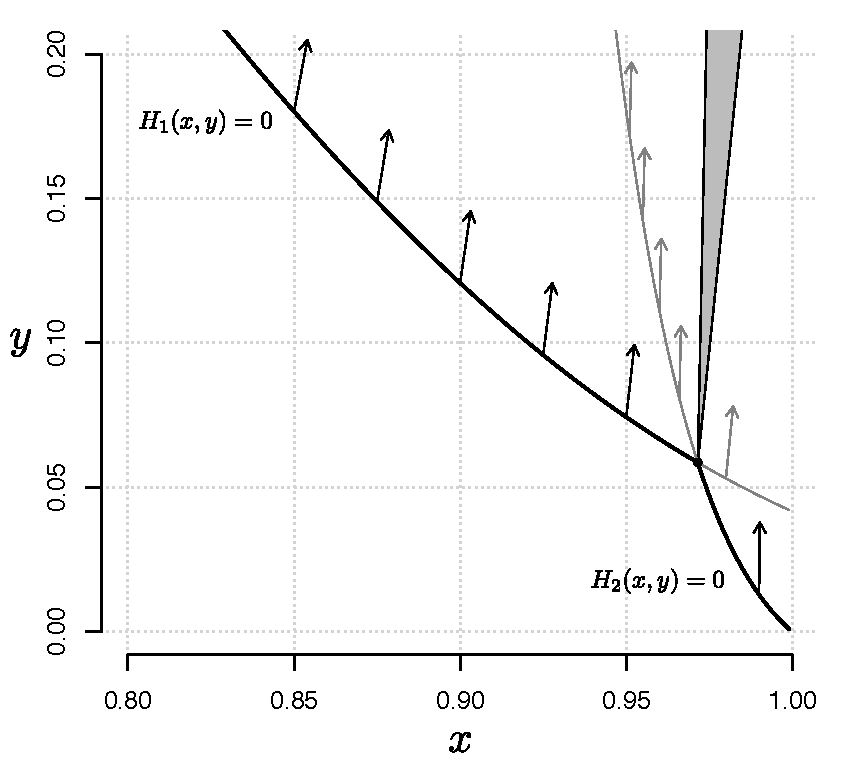
\includegraphics[scale=0.55]{Fig5.pdf}
%\caption{\textbf{Singular portrait of $K_1(x,y)$ for $d=24$}. The two
%curves labelled represent the points such that $H_1(x,y) = 0$ and
%$H_2(x,y) = 0$, respectively. The arrows indicate the ray associated with
%a critical point, and the grey triangle represents the cone of rays
%associated with the double point. The minimal critical points are shown in
%black, and the non minimal points in grey. Note that the $x$-axis does
%starts at 0.80.}
%\label{fig:singular}
%\end{figure}
%
%Figure~\ref{fig:singular} shows the critical points of $H(x,y)$ for
%$d=24$. The curves intersect at the point $\left( 1/2^{\frac{1}{d}},
%2^{1+\frac{1}{d}}-2 \right)$, which is the only double point, associated
%with the directions in the interval bounded below by $\lambda_- =
%(d-(d-1)2^{\frac{1}{d}}) / (2^{\frac{1}{d}}-1)$ and above by $\lambda_+ =
%(d2^{\frac{1}{d}}-d+1) / (2^{\frac{1}{d}}-1)$, indicated as a black
%triangle.  Smooth points are associated with a single direction computed
%from equation (\ref{eq:minimal}) and indicated by arrows.
%
%The asymptotics of the coefficients are governed by three regimes: if the
%direction $\lambda = \lim k/n$ is between $1$ and $\lambda_-$, the minimal
%critical point is a smooth point solution of $H_1(x,y) = 0$. If $\lambda$
%is between $\lambda_-$ and $\lambda_+$, the minimal critical point is the
%double point. If $\lambda$ is higher than $\lambda_+$ the minimal critical
%point is a smooth point solution of $H_2(x,y) = 0$. In words, the behavior
%is governed by $K(x,y)$ when $k/n$ is low, by $G(x,y)$ when $k/n$ is high,
%and by a combination of the two when $k/n$ is intermediate.
%
%\begin{proposition}
%Let the generating function of the array $(a_{k,n})$ be
%
%\begin{equation*}
%\frac{g(x,y)}{H(x,y)} =
%\frac{g(x,y)}{\prod_{i=1}^rH_i(x,y)}.
%\end{equation*}
%
%If the minimal critical point $(x,y)$ associated with the direction
%$\lambda = \lim k/n$ is smooth, then
%
%\begin{equation*}
%a_{k,n} \sim [x^ky^n] \frac{g(x,y)}{H_i(x,y)}\text{, where $i \leq r$ is
%such that } H_i(x,y) = 0.
%\end{equation*}
%
%If the minimal critical point is a double point, then
%
%\begin{equation*}
%\begin{split}
%a_{k,n} \sim \frac{1}{x^{k+1}y^{n+1}} \frac{g(x,y)}{\sqrt{-\mathcal{H}}}
%\text{, where} \\
%\mathcal{H} = \frac{\partial^2H(x,y)}{\partial x^2}
%  \frac{\partial^2H(x,y)}{\partial y^2} -
%\left( \frac{\partial^2H(x,y)}{\partial x\partial y} \right)^2.
%\end{split}
%\end{equation*}
%\end{proposition}
%
%When $\lim k/n < \lambda_-$, the number of configurations is
%asymptotically equivalent to the coefficients of
%
%\begin{equation*}
%\frac{yx(1-x^d)/(1-x)}{1-yx(1-x^d)/(1-x)}.
%\end{equation*}
%
%This case was studied in section \ref{subsec:closure}, so we can use
%algorithm \ref{alg:closure} to estimate the probability that the
%configuration contains exactly $1$ contig.
%
%When $\lambda_- \leq \lim k/n \leq \lambda_+$, the minimal critical point
%is the double point $\left( 1/2^{\frac{1}{d}}, 2^{1+\frac{1}{d}}-2
%\right)$ and the number of configurations is asymptotically proportional
%to $2^{\frac{k+1}{d}-n-1}/(2^{\frac{1}{d}}-1)^{n+1}$. Since
%$g(1/2^{\frac{1}{d}}, 2^{1+\frac{1}{d}}-2) = 1$, the proportionality
%constant is equal to $1/\sqrt{-\mathcal{H}}$.  Using the asymptotic
%formula for the total number of configurations, the probability that it
%contains exactly $1$ contig is asymptotically equivalent to
%
%\begin{equation}
%\label{eq:1contig_case2}
%\frac{(k/n)^k2^{\frac{k}{d}-n}}{(k/n-1)^{k-n} (2^{\frac{1}{d}}-1)^{n+1}}
%\sqrt{\frac{2\pi k(k/n-1)}{3(7d^2-6d+3)2^{\frac{2}{d}}-
%(3d^2-d)2^{1+\frac{1}{d}} +d^2 }}.
%\end{equation}
%
%Finally, when $\lim k/n > \lambda_+$, the number of configurations is
%asymptotically equivalent to the coefficients of
%
%\begin{equation*}
%\frac{yx(1-x^d)/(1-x)}{\left( 1-yx^{d+1}/(1-x) \right)^2}.
%\end{equation*}
%
%Observe that this generating function is related to the derivative of
%$G(x,y)$. More specifically
%
%\begin{equation*}
%\frac{\partial G(x,y)}{\partial y} =
%\frac{x^{d+1}/(1-x)}{\left( 1-yx^{d+1}/(1-x) \right)^2} =
%\frac{x^d}{1-x^d}\frac{yx(1-x^d)/(1-x)}{\left( 1-yx^{d+1}/(1-x)
%\right)^2}.
%\end{equation*}
%
%Thus, using equation (\ref{eq:m=0}), we can immediately give the asymptotic
%probability that the configuration contains exactly $1$ contig as
%
%\begin{equation}
%\label{eq:1contig_case3}
%\frac{n((k/n-d)^d-(k/n-d-1)^d)(k/n-1)^{k-n+\frac{1}{2}}
%(k/n-d)^{k-dn-\frac{1}{2}}}
%{(k/n)^{k-\frac{1}{2}}(k/n-d-1)^{k-(d+1)(n-1)-\frac{1}{2}}}.
%\end{equation}
%
%\begin{figure}[h]
%\centering
%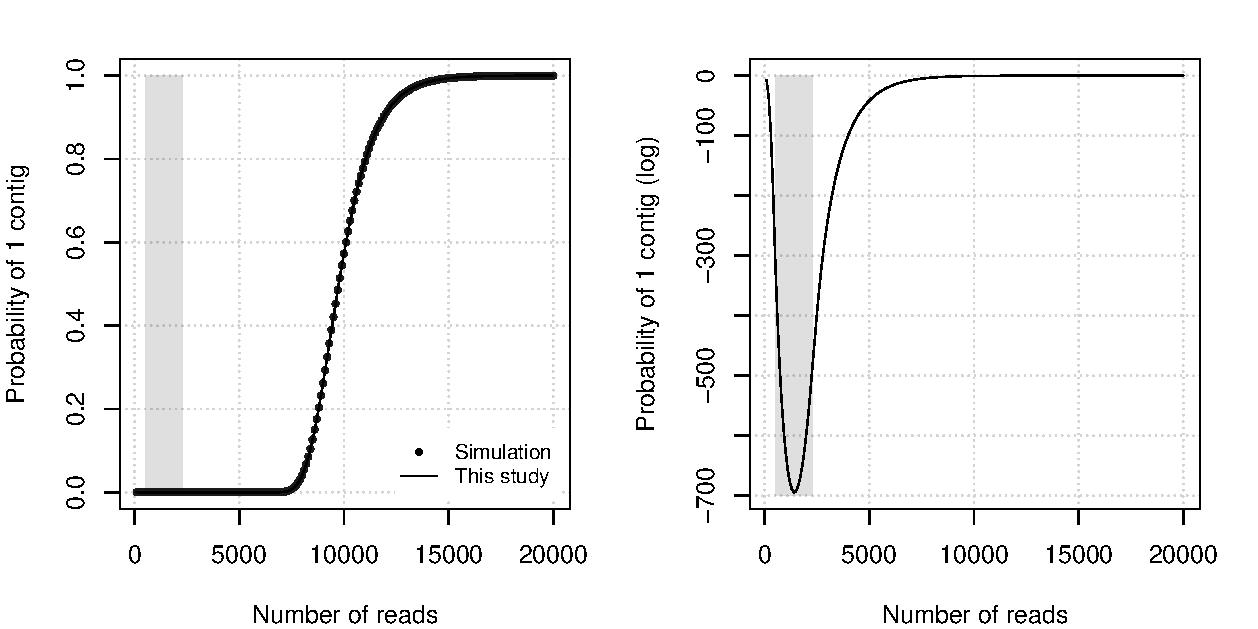
\includegraphics[scale=0.55]{Fig6.pdf}
%\caption{\textbf{Probability that the configuration has $1$ contig}.
%As in the previous examples, $k=25,000$ and $d=24$. Between $100$ and
%$20,000$ reads were drawn at random with replacement. Each case was
%replicated $500,000$ times and the average frequency that the
%configuration has exactly $1$ contig was plotted (circles). The plain
%lines show the estimate computed from algorithm \ref{alg:closure}, formula
%(\ref{eq:1contig_case2}) and forumla (\ref{eq:1contig_case3}).
%The grey shadow shows for which values the double point determines the
%asymptotics, \textit{i.e.} where formula (\ref{eq:1contig_case2}) was
%used. The estimate never deviates by more than 0.002. The right panel
%shows the logarithm of the estimate to highlight the asymptotic behavior
%at low coverage.}
%\label{fig:1contig}
%\end{figure}
%
